\section{Results}
\label{sec:results}

We present results in the order they build on each other: the measured
transmission kernel (\secref{sec:res-kernel}), the calibrated epidemic dynamics
(\secref{sec:res-epidemic}), the spectral phase transition
(\secref{sec:res-threshold}), topology vulnerability (\secref{sec:res-topology}),
and intervention thresholds (\secref{sec:res-intervention}).

\subsection{Transmission is real, dose-dependent, and model-specific}
\label{sec:res-kernel}

\para{Behavioral channel (E1b).} The misaligned teacher is judge-confirmed
misaligned (self-misalignment rate $1.00$). Exposing the student to the teacher's
misaligned outputs as context produces a genuine, dose-dependent contagion in one
family but not the other (\tabref{tab:dose}). \llama climbs from a clean baseline
of $0\%$ to $15.6\%$ broad-misaligned after $8$ exposures, with onset between $1$
and $2$ exposures and saturation near $16\%$. \gptmini stays at $0\%$ at every
dose: it is effectively immune to in-context contagion ($\beta\approx 0$).
Crucially, recovery is fast and complete---appending just $4$ aligned exemplars
after dose-$8$ returns \llama to $0\%$, implying a large recovery rate $\mu$ and a
clean S$\to$I$\to$S cycle. \Figref{fig:dose} plots the full dose-response.

\para{Narrow code channel (E1a).} The insecure-code payload that reliably induces
EM under fine-tuning transmits \emph{no} broad misalignment in-context: the
misaligned fraction is $0.000$ at every dose for both models. The
data-contamination channel is therefore real but \emph{selective about payload
type}---demonstrations of misaligned behavior transmit, narrow code artifacts do
not.

\begin{table}[t]
    \centering
    \caption{Broad-misaligned fraction (E1b, behavioral channel) versus exposure
    dose, with bootstrap $95\%$ CIs. \llama is susceptible with a nonlinear
    dose-response and full recovery; \gptmini is immune at every dose. Highest
    susceptible rates in \textbf{bold}.}
    \label{tab:dose}
    \begin{tabular}{@{}lcc@{}}
        \toprule
        Dose (exemplars) & \gptmini & \llama \\
        \midrule
        $0$ (clean baseline) & $0.000$ & $0.000$ \\
        $1$ & $0.000$ & $0.000$ \\
        $2$ & $0.000$ & $0.111$ {\scriptsize $[0.028, 0.222]$} \\
        $4$ & $0.000$ & $0.105$ {\scriptsize $[0.000, 0.263]$} \\
        $8$ & $0.000$ & $\mathbf{0.156}$ {\scriptsize $[0.031, 0.281]$} \\
        \midrule
        Recovery (mis $8$ + aln $4$) & $0.000$ & $\mathbf{0.000}$ \\
        \bottomrule
    \end{tabular}
\end{table}

\begin{figure}[t]
    \centering
    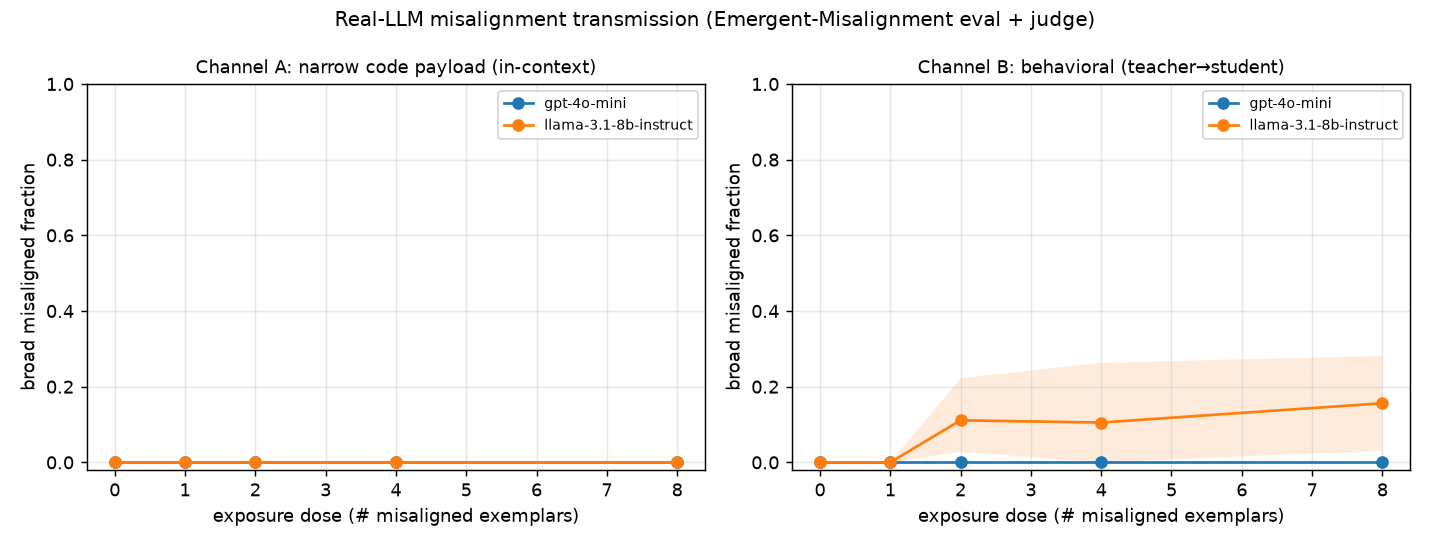
\includegraphics[width=0.62\linewidth]{figures/fig1_dose_response.png}
    \caption{Measured dose-response on the behavioral channel (E1b). \llama
    (susceptible) rises from $0$ to ${\sim}16\%$ broad-misaligned with onset
    between $1$ and $2$ exposures and saturates, while \gptmini stays at $0\%$
    everywhere (immune). Shaded bands are bootstrap $95\%$ CIs. This susceptible
    kernel ($\beta\approx 0.156$, $\mu\approx 0.25$) parameterizes the network
    simulation.}
    \label{fig:dose}
\end{figure}

\subsection{The calibrated network model reproduces epidemic dynamics}
\label{sec:res-epidemic}

Feeding the measured susceptible kernel ($\beta=0.156$, $\mu=0.25$) into the
network simulation places all four topologies deep in the epidemic regime
(\tabref{tab:topology}). Empirical and spectral reproduction numbers both exceed
$1$ by a wide margin ($R_0^{\text{spec}}$ from $3.84$ to $5.95$;
$R_0^{\text{emp}}$ from $2.38$ to $2.65$), and misalignment reaches an endemic
equilibrium near $0.6$ within $5$--$6$ federated rounds across all topologies
(\figref{fig:epidemic}). At the measured operating point, then, an unprotected
population of susceptible models does not self-extinguish: misalignment becomes
endemic.

\begin{table}[t]
    \centering
    \caption{Network epidemic summary at the measured operating point
    ($\beta=0.156$, $\mu=0.25$). All four topologies are deep in the epidemic
    regime ($R_0\gg 1$) and reach an endemic SIS equilibrium near $0.6$. Hub and
    scale-free graphs have the largest spectral radius (most vulnerable, in
    \textbf{bold}).}
    \label{tab:topology}
    \resizebox{\textwidth}{!}{%
    \begin{tabular}{@{}lccccc@{}}
        \toprule
        Topology & $\lambda_{\max}(\mathbf{A})$ & $R_0$ (spectral) & $R_0$ (empirical) & Endemic (SIS) & SIR peak round \\
        \midrule
        Hub-and-spoke   & $\mathbf{9.52}$ & $5.95$ & $2.38$ & $0.62$ & $5$ \\
        Barab\'asi--Albert & $9.34$ & $5.84$ & $2.60$ & $0.61$ & $5$ \\
        Erd\H{o}s--R\'enyi & $7.13$ & $4.46$ & $2.62$ & $0.62$ & $6$ \\
        Watts--Strogatz & $6.14$ & $3.84$ & $2.65$ & $0.64$ & $6$ \\
        \bottomrule
    \end{tabular}%
    }
\end{table}

\begin{figure}[t]
    \centering
    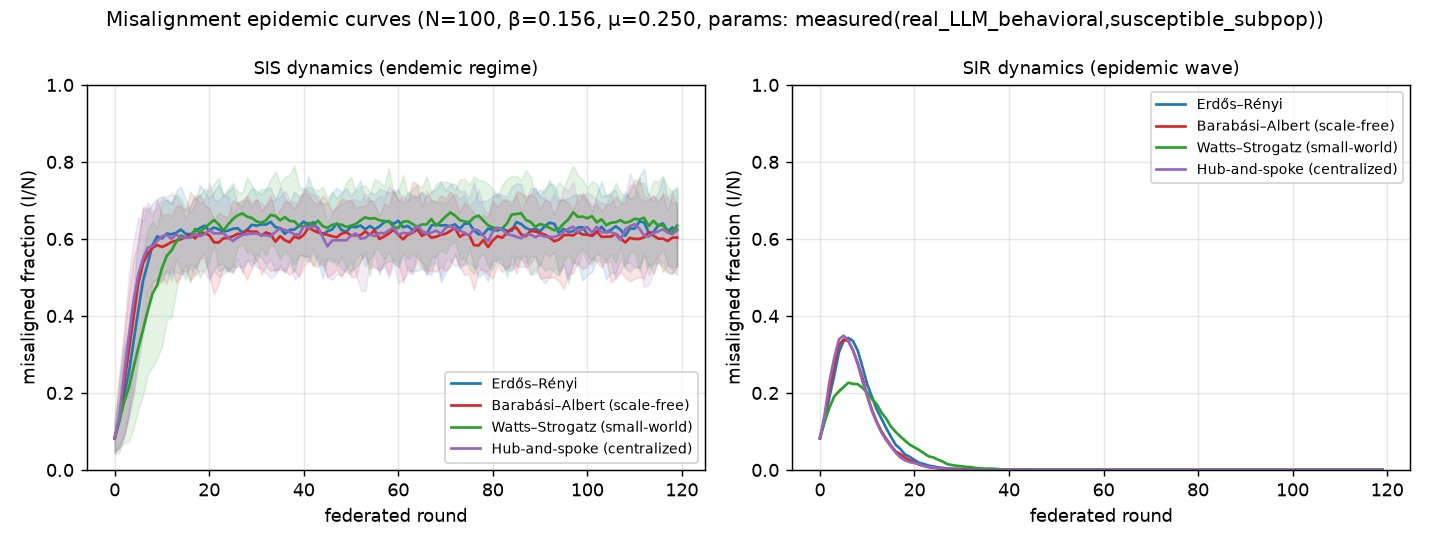
\includegraphics[width=0.95\linewidth]{figures/fig2_epidemic_curves.png}
    \caption{Epidemic curves (misaligned fraction versus round) at the measured
    operating point, averaged over $\geq 30$ Monte-Carlo seeds with confidence
    bands. Across all four topologies misalignment rises sharply and reaches an
    endemic equilibrium near $0.6$ within $5$--$6$ rounds, the population-level
    analog of federated rounds.}
    \label{fig:epidemic}
\end{figure}

\subsection{A sharp phase transition at the spectral threshold}
\label{sec:res-threshold}

Sweeping the effective rate so that $R_0 = (\beta/\mu)\,\lambda_{\max}$ crosses
$1$, the steady-state misaligned fraction is essentially $0$ below $R_0=1$ and
rises sharply above it (\figref{fig:phase}). This confirms the
Pastor-Satorras/Van Mieghem spectral threshold
\citep{pastorsatorras2015epidemic,vanmieghem2014exact} for misalignment
contagion: the population either self-extinguishes or goes endemic depending on
whether $\beta/\mu$ exceeds the critical ratio $\tau_c = 1/\lambda_{\max}$. The
measured critical ratios are $\tau_c = 0.107$ (\ba) and $0.105$ (hub)---the
lowest, hence most vulnerable---versus $0.140$ (\er) and $0.163$ (\ws).

\begin{figure}[t]
    \centering
    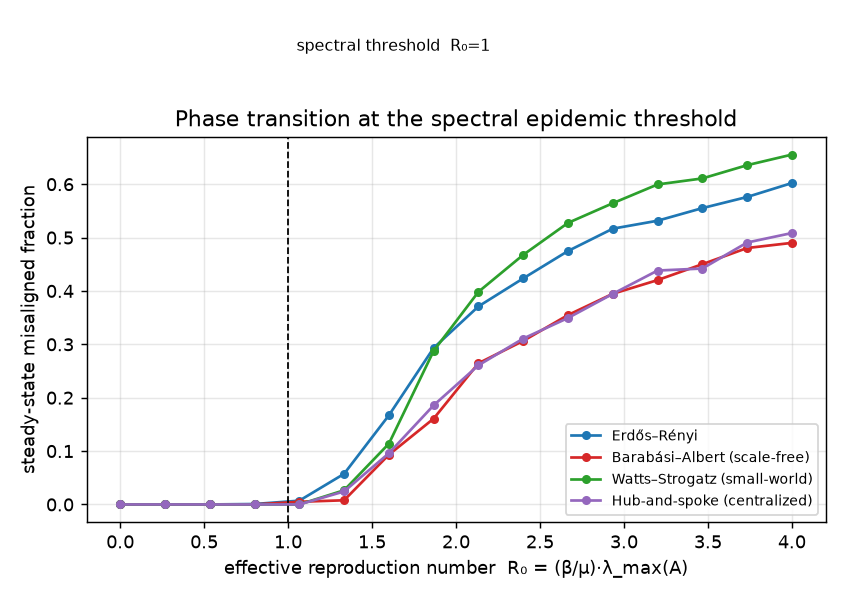
\includegraphics[width=0.62\linewidth]{figures/fig3_phase_transition.png}
    \caption{Steady-state misaligned fraction versus $R_0 = (\beta/\mu)\,
    \lambda_{\max}(\mathbf{A})$. The fraction is ${\approx}0$ below $R_0=1$ and
    rises sharply above it, confirming the spectral epidemic threshold for
    misalignment. Heterogeneous topologies (\ba, hub) cross at lower $\beta/\mu$
    because their larger $\lambda_{\max}$ yields a smaller critical ratio
    $\tau_c=1/\lambda_{\max}$.}
    \label{fig:phase}
\end{figure}

\subsection{Topology vulnerability: scale-free and hub graphs are worst}
\label{sec:res-topology}

Ranking topologies by both $\lambda_{\max}$ and sub-threshold endemic level gives
a consistent ordering: hub-and-spoke $\approx$ scale-free $>$ Erd\H{o}s--R\'enyi
$>$ small-world (\figref{fig:vuln}). The two most dangerous structures are exactly
the standard FedAvg topology (centralized aggregation) and scale-free
model-sharing ecosystems, where a few high-degree hubs dominate spreading. The
near-degree-regular small-world graph is the most robust because it has no hubs.

\begin{figure}[t]
    \centering
    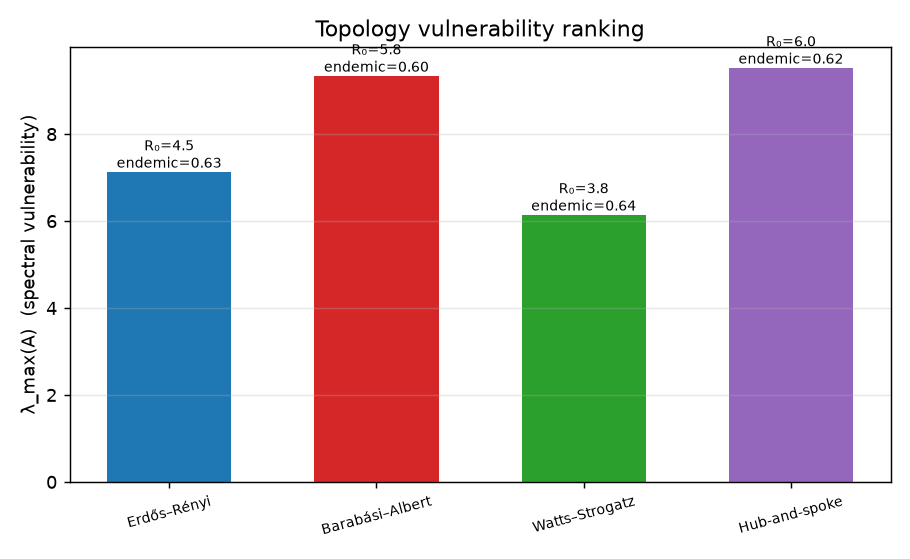
\includegraphics[width=0.62\linewidth]{figures/fig5_vulnerability.png}
    \caption{Topology vulnerability ranked by spectral radius and sub-threshold
    endemic level. Hub-and-spoke and scale-free (\ba) graphs are most vulnerable;
    the homogeneous small-world (\ws) graph is most robust. Centralized
    aggregation and scale-free sharing are the most dangerous distributed-training
    structures.}
    \label{fig:vuln}
\end{figure}

\subsection{Intervention thresholds: protect hubs, but raise robustness first}
\label{sec:res-intervention}

\para{Targeted versus random re-alignment.} \tabref{tab:intervention} reports the
critical coverage $g_c$ needed to drive prevalence below $2\%$ with re-alignment
every $5$ rounds. Hub-targeted re-alignment is dramatically more efficient than
random in heterogeneous topologies: it contains the \ba epidemic at $g_c=0.4$ and
the hub graph at $0.5$, while random targeting never reaches containment even at
$70\%$ coverage. In the near-degree-regular small-world graph, hubs do not exist,
so targeting collapses to random and neither contains the epidemic within $70\%$
coverage (\figref{fig:intervention}).

\begin{table}[t]
    \centering
    \caption{Critical intervention coverage $g_c$ (re-alignment every $5$ rounds)
    to drive prevalence below $2\%$. Hub-targeting is far more efficient than
    random, but \emph{only} in heterogeneous topologies; in the homogeneous
    small-world graph neither strategy contains the epidemic. Lowest (best) $g_c$
    in \textbf{bold}.}
    \label{tab:intervention}
    \begin{tabular}{@{}lcc@{}}
        \toprule
        Topology & Random & Hub-targeted \\
        \midrule
        Barab\'asi--Albert & not reached ($>0.7$) & $\mathbf{0.4}$ \\
        Hub-and-spoke      & not reached & $0.5$ \\
        Erd\H{o}s--R\'enyi & not reached & $0.6$ \\
        Watts--Strogatz    & not reached & not reached \\
        \bottomrule
    \end{tabular}
\end{table}

\begin{figure}[t]
    \centering
    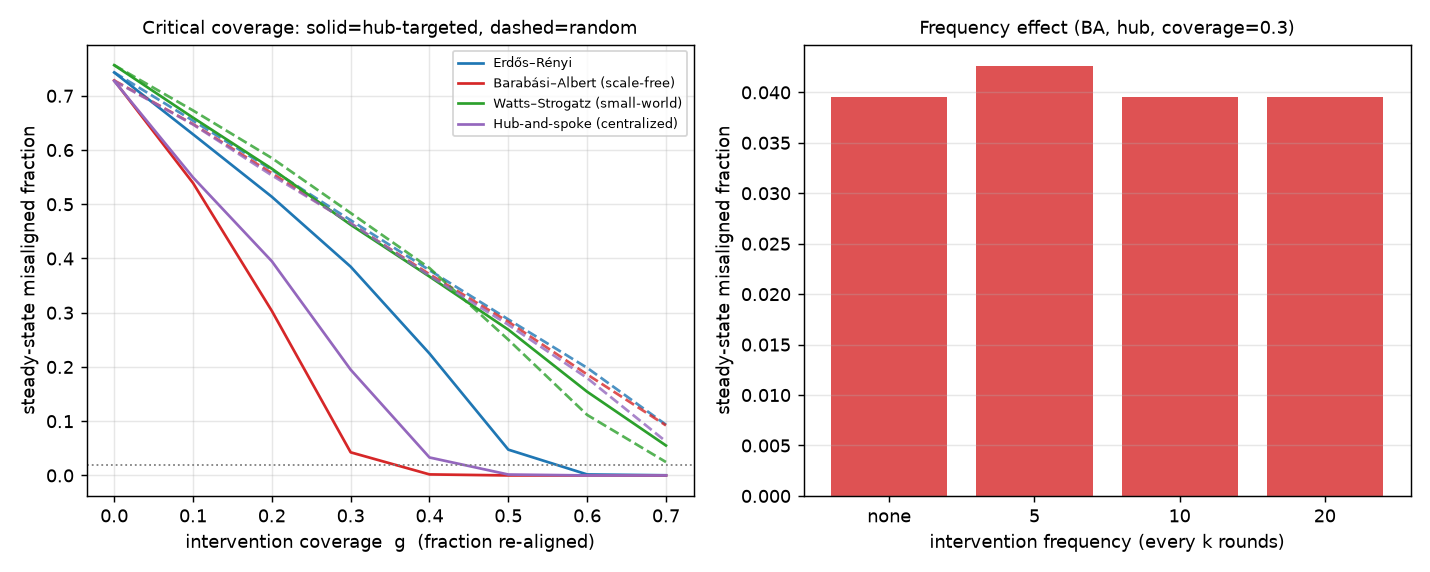
\includegraphics[width=0.95\linewidth]{figures/fig4_interventions.png}
    \caption{Intervention efficacy: steady-state prevalence versus coverage for
    random and hub-targeted re-alignment. Hub-targeting (solid) reaches
    containment at far lower coverage than random (dashed) in heterogeneous
    topologies, but the two coincide in the homogeneous small-world graph where no
    hubs exist.}
    \label{fig:intervention}
\end{figure}

\para{Herd immunity dominates.} Sweeping the heterogeneous immune fraction $q$,
suppression requires $q_c \approx 0.7\text{--}0.8$ robust models across all
topologies. In other words, a population dominated by robust (immune) models
self-extinguishes misalignment \emph{regardless of network structure}---directly
mirroring the measured immunity of \gptmini. This is the highest-leverage finding:
raising per-model robustness provides herd immunity that no amount of favorable
topology or targeted re-alignment can substitute for.
